\subsubsection{13.04.15}
\begin{enumerate}
	
	\item The time of beginning and ending of the meeting: 17:00 - 23:00.
	
	\item Purposes of the meeting: 
	\begin{enumerate}
		
		\item To finish the wheel base.
		
		\item To fix MEL.
		
		\item To install stoppers on the rails.
		
		\item To test the robot.
		
	\end{enumerate}
	
	\item Work that has been done:
	\begin{enumerate}
				
		\item MEL was fixed.
		\begin{figure}[H]
			\begin{minipage}[h]{0.2\linewidth}
				\center  
			\end{minipage}
			\begin{minipage}[h]{0.6\linewidth}
				\center{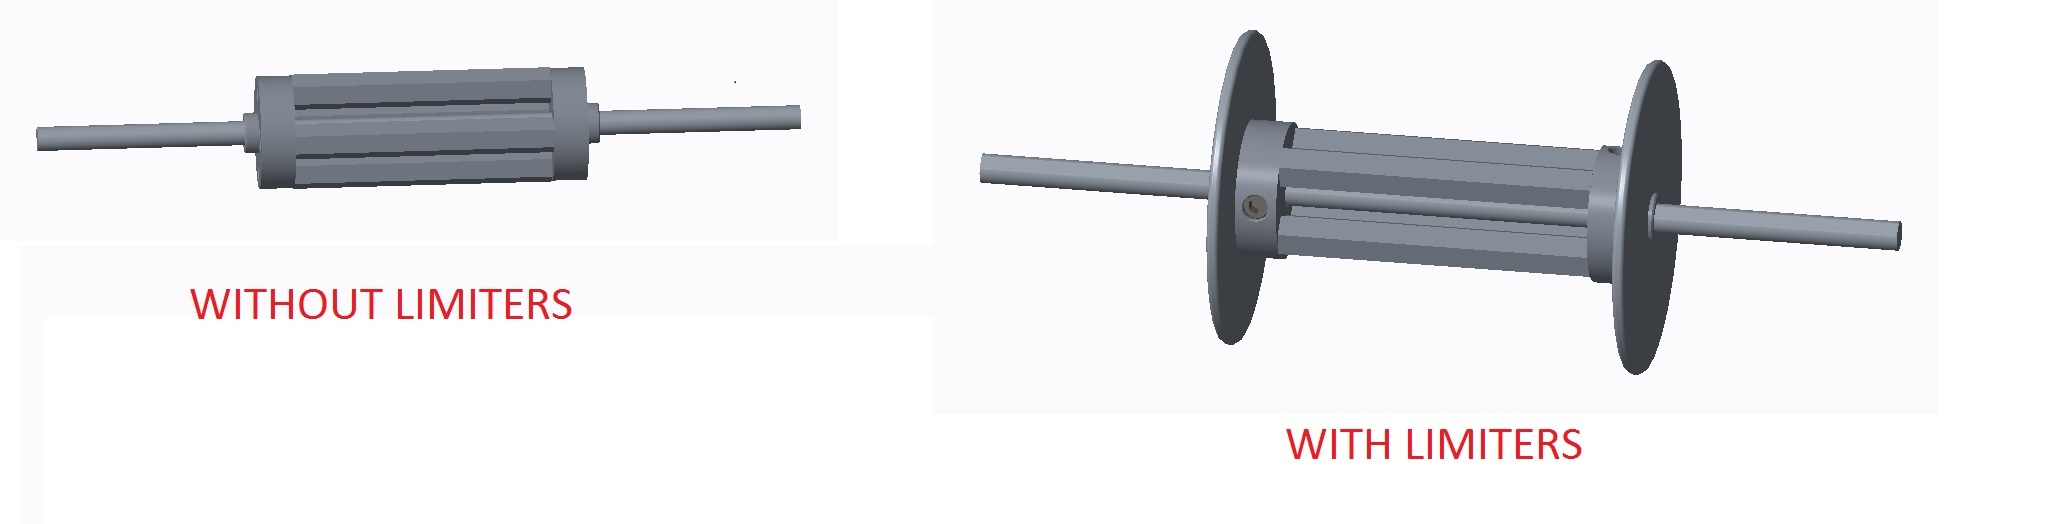
\includegraphics[scale=0.3]{days/07.04.15/images/01}}
				\caption{}
			\end{minipage}
		\end{figure}
		
		\item It was decided to connect the top crossbars with each other by the rope. It will not allow the bottom crossbars lift too high.
		\begin{figure}[H]
			\begin{minipage}[h]{0.2\linewidth}
				\center  
			\end{minipage}
			\begin{minipage}[h]{0.6\linewidth}
				\center{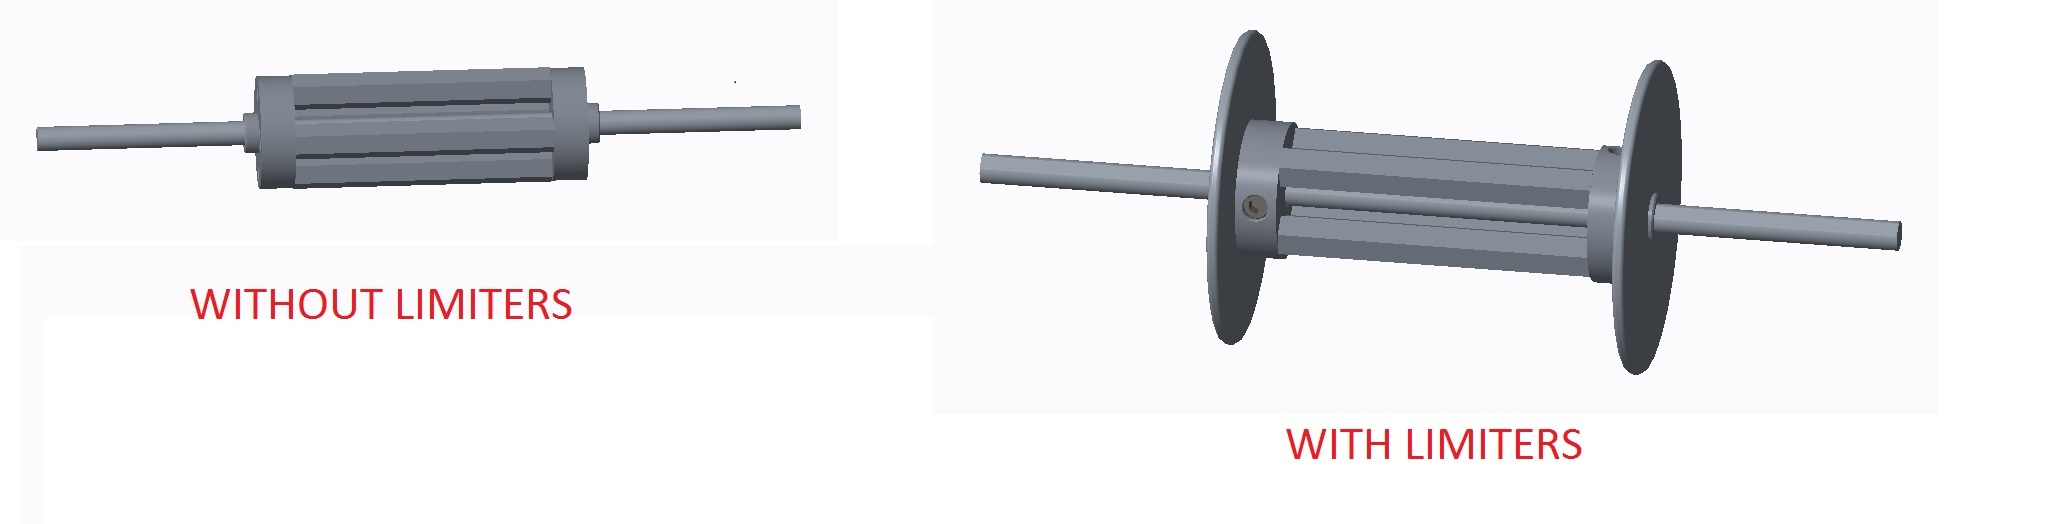
\includegraphics[scale=0.3]{days/07.04.15/images/01}}
				\caption{}
			\end{minipage}
		\end{figure}
		
		\item Wheel base was tested. It was turned out that robot can't turn on our field. Most likely it happened due to other arrangement of the wheels (compared with what we had on the "Robofest"). When we had old wheel base our robot turned on our field due to the back wheels and front wheels slip (In the original field robot turned normaly because there is lower friction on the original field). Now all wheel are not slip and due to high friction robot can't turn. It not allow us to train before competition. So we need to change wheel base.
		
		\item We tryed to wrap wheels with electrical tape. Tape is more slippery and so it can to help us. But robot still didn't turn.
		
		\item We looked the variant to install Lego tires on the wheels but they were too small.
		
		\item It was decided to install omni-wheels instead of standard. This variant was tested. Result is positive. Robot move and turn very fast. Also it ride to the ramp almost without problems. There was only one problem that when we ride to the ramp not directly but at an angle robot slip from it due to rollers. But we think that it not very big problem.
		
		\item Also we looked a variant to install Lego caterpillars on the wheels but we decided that construction with omni-wheels is better because robot with omni-wheels can turn faster and more accurate.
		
		\item It was decided to install beam that will connect axles of two wheels. It will not allow to gears move away from each other. So we need to move wheels closer to the beam of the base. The right wheels were moved on the desired distance.  
		
	\end{enumerate}
	
	\item Results:
	\begin{enumerate}
		
		\item MEL was fixed. 
		
		\item Limiters for lift were projected.
		
		\item Wheel base was changed and tested.
		
	\end{enumerate}
	
	\item Tasks for the next meetings:
	\begin{enumerate}
		
		\item To install beams thet connect two wheels with each other.
		
		\item To install limiters on the lift.
		
		\item To install button of power with Lego motor.
		
	\end{enumerate}
\end{enumerate}
\fillpage
